\documentclass[
	ngerman,
	%twoside,
	BCOR=8mm,
	headings=normal,
	parskip=half,
	headsepline,
	automark,
	listof=totoc,
	bibliography=totoc,
	%,captions=tableabove
	%draft
]{scrreprt}
%
%
\input{packages}
%
\input{definitions}
%
%%%%%%%%%%%%%%%%%%%%%%%%%%%%%%%%%%%%%%%%%%%%%%%%%%%%%%%%%%%%%%%%%%%%%%%%%%%%%%%
% Begriffe für glossaries definieren
%%%%%%%%%%%%%%%%%%%%%%%%%%%%%%%%%%%%%%%%%%%%%%%%%%%%%%%%%%%%%%%%%%%%%%%%%%%%%%%

%=== Glossar ==================================================================
\newglossaryentry{gls:embedding}{
	name={Embedding},
	description={Abbildung eines Datenobjekts wie Text oder Bild auf einen
	hochdimensionalen Vektor, dessen geometrische Nähe semantische Ähnlichkeit
	widerspiegelt}
}

\newglossaryentry{gls:quantisierung}{
	name={Quantisierung},
	description={Reduktion der Darstellungsgenauigkeit eines Vektors, indem
	kontinuierliche Werte auf eine endliche Anzahl diskreter Stufen mit weniger
	Bits pro Dimension abgebildet werden}
}

\newglossaryentry{gls:binarisierung}{
	name={Binarisierung},
	description={Extremfall der Quantisierung, bei dem jede Dimension anhand
	ihres Vorzeichens auf ein einzelnes Bit reduziert wird}
}

\newglossaryentry{gls:distortion}{
	name={Distortion},
	description={Maß für die Verzerrung, die durch die Kompression zwischen
	dem Originalraum und dem rekonstruierten Raum entsteht}
}

\newglossaryentry{gls:paretofront}{
	name={Pareto-Front},
	description={Menge der nicht dominierten Konfigurationen, für die keine
	andere Konfiguration zugleich einen geringeren Speicherbedarf und eine
	höhere Qualität erreicht}
}

%=== Abkürzungen ==============================================================
\newacronym{ndcg}{NDCG}{Normalized Discounted Cumulative Gain}
\newacronym{dcg}{DCG}{Discounted Cumulative Gain}
\newacronym{mrr}{MRR}{Mean Reciprocal Rank}
\newacronym{beir}{BEIR}{Benchmarking Information Retrieval}
\newacronym{mteb}{MTEB}{Massive Text Embedding Benchmark}
\newacronym{pca}{PCA}{Principal Component Analysis (Hauptkomponentenanalyse)}
\newacronym{mrl}{MRL}{Matryoshka Representation Learning}
\newacronym{pq}{PQ}{Product Quantization}
\newacronym{ann}{ANN}{Approximate Nearest Neighbor}
\newacronym{blas}{BLAS}{Basic Linear Algebra Subprograms}
\newacronym{rag}{RAG}{Retrieval-Augmented Generation}
\newacronym{twonn}{TwoNN}{Two Nearest Neighbors}
\newacronym{aws}{AWS}{Amazon Web Services}
\newacronym{ec2}{EC2}{Elastic Compute Cloud}

%=== Symbole ==================================================================
\newglossaryentry{sym:dim}{
	name={\ensuremath{d}},
	description={Dimensionszahl der Vektorrepräsentation},
	type=symbols,
}

\newglossaryentry{sym:dimint}{
	name={\ensuremath{d_\text{int}}},
	description={Intrinsische Dimensionalität, effektive Anzahl unabhängiger
	Freiheitsgrade des Datenraums},
	type=symbols,
}

\newglossaryentry{sym:N}{
	name={\ensuremath{N}},
	description={Anzahl der Vektoren im Index beziehungsweise Korpus},
	type=symbols,
}

\newglossaryentry{sym:k}{
	name={\ensuremath{k}},
	description={Größe der betrachteten Nachbarschaft oder Position des
	Rang-Cutoffs bei Retrieval-Metriken},
	type=symbols,
}

\newglossaryentry{sym:pearson}{
	name={\ensuremath{r}},
	description={Pearson-Korrelationskoeffizient, misst den linearen
	Zusammenhang zwischen Distanzen},
	type=symbols,
}

\newglossaryentry{sym:spearman}{
	name={\ensuremath{\rho}},
	description={Spearman-Rangkorrelationskoeffizient, misst die
	Rangerhaltung von Distanzen},
	type=symbols,
}

\newglossaryentry{sym:cq}{
	name={\ensuremath{CQ_1}},
	description={Compression-Quality-Score, kombiniert Qualitätserhaltung und
	Speicherersparnis zu einer skalaren Trade-off-Kennzahl},
	type=symbols,
}

\newglossaryentry{sym:bitvektor}{
	name={\ensuremath{\mathbf{b}}},
	description={Binärer Vektor aus \ensuremath{\{0,1\}^d}, Ergebnis der
	Binarisierung},
	type=symbols,
}

\newglossaryentry{sym:memory}{
	name={\ensuremath{M(N)}},
	description={Speicherbedarf eines Index mit \ensuremath{N} Vektoren},
	type=symbols,
}

%
\makeglossaries
%
\graphicspath{{images/}}
%
\addbibresource{references.bib}

\nocite{*} % listet alle Quellen (auch die nicht zitierten!)
%
%=== für schnelleres kopilieren alle ungeänderten Dateien auskommentieren =====
\includeonly{
	content/chapDeclaration,
	content/chapAbstract,
	content/chapEinleitung,
	content/chapGrundlagen,
	content/chapMethodik,
	content/chapErgebnisse,
}
%
%
%==============================================================================
%
\begin{document}
%
\pdfbookmark[0]{Titelseite}{titel}
\begin{titlepage}
%
\sffamily% Umschalten auf serifenlose Schrift
%
\begin{center}
\begin{tikzpicture}
 \fill[THRed] (0, 0) rectangle (\textwidth/3, 3pt);
 \fill[THOrange] (\textwidth/3, 0) rectangle (2*\textwidth/3, 3pt);
 \fill[THPurple] (2*\textwidth/3, 0) rectangle (\textwidth, 3pt);
\end{tikzpicture}
\end{center}
%
\vfill
%
\begin{huge}
Bit statt Float? Eine vergleichende Untersuchung binärer und kontinuierlicher Embeddings für semantisches Retrieval\\[10mm]
\end{huge}
%
Projektarbeit\newline
zum Modul \emph{Deep Learning, Machine Learning und Künstliche Intelligenz}\newline
im Studiengang Informatik\newline
an der Fakultät für Informatik und Ingenieurwissenschaften\newline
der Technischen Hochschule Köln
%
\vfill
%
\begin{tabular}{@{}ll}
vorgelegt von: & Nick Betker\\
               & Nils Morczinietz\\
               & Jesko Förster\\[5mm]
eingereicht bei:   & Prof. Dr. Daniel Gaida\\
\end{tabular}	
%
\\[10mm]
%
Gummersbach, TT.MM.JJJJ%
%
\rmfamily% Umschalten auf Standard-Schrift mit Serifen
%
\end{titlepage}
\cleardoublepage
\pagenumbering{Roman}
\chapter*{Kurzfassung}
\label{chap:abstract}

Embedding-basierte Vektorsuchsysteme bilden das Rückgrat moderner Informationsrückgewinnung und agentenbasierter KI-Architekturen. Mit wachsenden Dokumentkorpora steigen Speicherbedarf und Betriebskosten hochdimensionaler Float32-Vektoren jedoch drastisch an. Die nachträgliche Quantisierung auf wenige Bits pro Dimension verspricht erhebliche Speichervorteile, führt jedoch unweigerlich zu Informationsverlusten. 

In dieser Arbeit wird der Einfluss von Quantisierung und Dimensionsreduktion auf die Retrieval-Qualität und den Ressourcenbedarf systematisch und kausal untersucht. Anhand eines kontrollierten Sechs-Phasen-Experiments auf Basis des Embedding-Modells \texttt{bge-large-en-v1.5} und dreier heterogener BEIR-Datensätze (SciFact, FiQA, TREC-COVID) wird die Erhaltung geometrischer Raumeigenschaften, Distanzkorrelationen, Nachbarschaften und Retrieval-Metriken (NDCG@10, Recall@100) über verschiedene Bittiefen (1 bis 8~Bit) sowie PCA-Zielstufen evaluiert. Verglichen werden naive Quantisierungsansätze mit dem rotationsbasierten Verfahren TurboQuant.

Die Ergebnisse zeigen, dass eine Kompression bis 4-Bit praktisch verlustfrei bleibt und über 99{,}5\,\% der Float32-Retrieval-Qualität bei einer Speicherreduktion um das 7{,}8-Fache wahrt. Für kostenoptimierte Cloud-Systeme bietet 2-Bit bei voller Dimension (1024d) den besten Kompromiss mit 98{,}1\,\% erhaltener Qualität und 15-facher Speicherersparnis, was unter den gewählten Annahmen einer modellierten AWS-Infrastruktur 93{,}7\,\% der monatlichen Instanzkosten einspart. Selbst 1-Bit-Konfigurationen behalten eine hohe Trustworthiness und eignen sich für zweistufige Filterstrukturen sowie lokale On-Device-Szenarien mit 100\,000 bis 500\,000 Vektoren unterhalb von 50~MiB Arbeitsspeicher. Die geometrische Analyse belegt zudem, dass TurboQuant durch orthogonale Rotation das bei nativer Binarisierung auftretende Verdünnungsparadox unter Dimensionsreduktion erfolgreich verhindert.

\vspace{0.5cm}
\noindent\textbf{Schlagwörter:} Vektor-Embeddings, Quantisierung, TurboQuant, Semantische Suche, Information Retrieval, Matryoshka-Reduktion, Skalierbarkeit

\cleardoublepage
\pdfbookmark[0]{Inhaltsverzeichnis}{toc}
\tableofcontents
\glsaddall
\listoftables
\listoffigures
\printglossary
\printglossary[type=\acronymtype, title={Abkürzungsverzeichnis}]
\printglossary[type=symbols, title={Symbolverzeichnis}]
%
\cleardoublepage
\KOMAoptions{open=right}
\pagenumbering{arabic}
\chapter{Einleitung}
%
Embedding-basierte Suchsysteme sind ein zentraler Baustein moderner KI-Anwendungen.
Sie werden unter anderem für semantische Suche, Retrieval-Augmented Generation (RAG) und Ähnlichkeitssuche eingesetzt.
In solchen Systemen werden Texte, Dokumente oder andere Datenobjekte als hochdimensionale Vektoren repräsentiert, deren Speicherung und Vergleich bei großen Datenmengen erhebliche Rechen- und Speicherressourcen erfordern.
Gleichzeitig wächst der praktische Bedarf an Systemen, die auch auf begrenzter Hardware schnell, speichereffizient und möglichst präzise arbeiten.
Besonders deutlich wird diese Anforderung im Kontext agentenbasierter KI-Systeme, die über standardisierte Protokolle wie das Model Context Protocol (MCP) \cite{anthropic_2024_mcp} auf externe Werkzeuge zugreifen und dabei Echtzeit-Retrieval unter strikten Latenzanforderungen benötigen.
\par
Die vorliegende Projektarbeit untersucht daher die Frage, wie sich Embeddings verändern, wenn anstelle klassischer Float-Vektoren stark komprimierte Bit- beziehungsweise Niedrigbit-Repräsentationen verwendet werden.
Aktuelle Entwicklungen zeigen, dass diese Richtung nicht nur theoretisch interessant ist, sondern auch praktisch relevant.
Google Research beschreibt mit TurboQuant eine Methode, die Vektoren mittels Rotation und skalaren Quantisierern auf wenige Bits pro Dimension komprimiert und dabei sowohl Distortion als auch Retrieval-Qualität günstig beeinflussen soll \cite{zandieh_2025_turboquant}; das Open-Source-Projekt turbovec setzt diesen Ansatz als Vektorindex mit Python-Anbindung um \cite{turbovec_2024}.
Parallel dazu zeigen Matryoshka-Embeddings, dass Modelle so trainiert werden können, dass auch reduzierte Embedding-Dimensionen noch leistungsfähig bleiben \cite{kusupati_2022_matryoshka}.
\par
Aus dieser Ausgangslage ergibt sich die zentrale Forschungsfrage der Arbeit:
Welche semantischen Eigenschaften eines Float-Embedding-Raums bleiben unter Quantisierung erhalten, welche gehen verloren, und wie wirkt sich dieser Verlust auf die Retrieval-Qualität aus?
Der Fokus liegt damit nicht auf einer bloßen Implementierung eines weiteren Suchsystems, sondern auf dem wissenschaftlichen Verständnis, \emph{warum} bestimmte Kompressionsverfahren auf bestimmten Daten besser oder schlechter funktionieren und welche praktischen Konsequenzen sich daraus ergeben.
Um die gewonnenen Erkenntnisse über einen isolierten Benchmark hinaus zu validieren, werden die untersuchten Retrieval-Systeme zusätzlich als MCP-Server bereitgestellt und in einem realistischen Anwendungsszenario evaluiert.
Die Arbeit entwickelt dabei keine neuen Quantisierungsverfahren und trainiert keine spezialisierten Embedding-Modelle, sondern analysiert den Informationsverlust bestehender Methoden auf einem kontrollierten Float-Referenzraum und prüft deren praktische Einsetzbarkeit in einer agentenbasierten Architektur.

\chapter{Grundlagen}
\label{chap:grundlagen}
%
\section{Embeddings und vektorbasierte Suche}
%
Embeddings dienen dazu, semantische Information in einen numerischen Vektorraum zu überführen.
Ob zwei Objekte ähnlich sind, wird nicht über exakte Zeichenfolgen oder Regeln bestimmt, sondern über die geometrische Nähe ihrer Vektoren.
In der Praxis werden dafür meist Float-Vektoren verwendet, typischerweise in 384, 768 oder 1536 Dimensionen.
%
Das gebräuchlichste Ähnlichkeitsmaß für Embedding-Vektoren ist die Cosine-Similarity:
\begin{equation}
  \text{cos}(\mathbf{x}, \mathbf{y}) = \frac{\mathbf{x} \cdot \mathbf{y}}{\|\mathbf{x}\|_2 \cdot \|\mathbf{y}\|_2}
\end{equation}
%
Sie misst den Winkel zwischen zwei Vektoren, unabhängig von deren Länge.
Werte nahe~1 bedeuten hohe semantische Ähnlichkeit, Werte nahe~0 Unabhängigkeit.
Für normierte Vektoren ($\|\mathbf{x}\|_2 = 1$) vereinfacht sich die Cosine-Similarity zum Skalarprodukt, was die Berechnung beschleunigt.
%
Float-Repräsentationen sind flexibel und präzise, verursachen aber bei großen Korpora erhebliche Speicher- und Suchkosten.
Ein Korpus von 10 Millionen Dokumenten benötigt als Float32-Vektoren mit 768 Dimensionen rund 31~GB RAM.
Jede Ähnlichkeitsberechnung erfordert 768 Multiplikationen und Additionen.
Bei Brute-Force-Suche skaliert die Suchzeit linear mit der Korpusgröße, was für Echtzeit-Anwendungen schnell unpraktikabel wird.
%
\section{Quantisierung}
%
Quantisierung bezeichnet die Abbildung eines kontinuierlichen Wertebereichs auf eine endliche Menge diskreter Stufen, ein Grundproblem der Informationstheorie, das bereits in Shannons Rate-Distortion-Theorie \cite{shannon_1959_ratedistortion} formalisiert wurde.
Im Kontext von Embeddings bedeutet dies, dass jede Dimension eines Vektors statt mit 32~Bit (Float32) mit weniger Bits dargestellt wird.
%
Der Informationsverlust bei Quantisierung ist unvermeidlich.
Werden $n$ Werte auf $k < n$ Stufen abgebildet, gehen Unterscheidungen verloren.
Die zentrale Frage ist nicht, \emph{ob} Information verloren geht, sondern \emph{welche} und ob die für eine Anwendung relevante Struktur erhalten bleibt.
%
Zwei Eigenschaften bestimmen die Qualität einer Quantisierung:
\begin{itemize}
  \item \textbf{Distortion}, also die mittlere Verzerrung der Distanzen zwischen Vektoren. Niedrige Distortion bedeutet, dass die geometrische Struktur des Raums weitgehend erhalten bleibt.
  \item \textbf{Distanzerhaltung der Rangordnung}, also ob die relative Reihenfolge der Ähnlichkeiten korrekt bleibt. Für Retrieval-Anwendungen ist diese Eigenschaft wichtiger als absolute Distanztreue, da nur das Ranking der Suchergebnisse relevant ist.
\end{itemize}
%
\section{Binäre Embeddings und Hamming-Distanz}
%
Die extremste Form der Quantisierung reduziert jede Dimension auf ein einzelnes Bit.
Die naive Variante nutzt das Vorzeichen:
positive Werte werden zu~1, negative oder Null zu~0.
Der resultierende Bitvektor benötigt pro Dimension nur $\frac{1}{32}$ des Speichers eines Float32-Vektors.
%
Die Ähnlichkeit zweier binärer Vektoren wird über die Hamming-Distanz bestimmt, also die Anzahl der Bitpositionen, an denen sich die Vektoren unterscheiden.
Diese Operation lässt sich auf moderner Hardware durch XOR und Population-Count in wenigen Taktzyklen berechnen, was Geschwindigkeitsvorteile um Größenordnungen gegenüber Float-Cosine ermöglicht.
%
Der Nachteil ist der potenzielle Informationsverlust.
Die Binarisierung verwirft sowohl die Magnitude jeder Dimension als auch die Norminformation des Gesamtvektors.
Ob dieser Verlust für eine gegebene Anwendung tolerierbar ist, hängt davon ab, wie viel semantische Information im Vorzeichen konzentriert ist. Die vorliegende Arbeit untersucht genau diese Frage empirisch.
%
\section{TurboQuant}
%
TurboQuant \cite{zandieh_2025_turboquant} adressiert das Spannungsfeld zwischen Kompaktheit und Genauigkeit über eine Quantisierung in zwei Schritten, die keine Trainingsphase auf den Zieldaten erfordert:
%
\begin{enumerate}
  \item \textbf{Rotation:} Die Eingabevektoren werden mit einer zufälligen orthogonalen Matrix multipliziert. Diese Rotation verändert die semantische Information nicht (Winkel und Abstände bleiben identisch), dekorreliert aber die Dimensionen. Nach der Rotation sind die Werte gleichmäßiger über die Dimensionen verteilt, sodass ein uniformer Quantisierer jede Dimension gleich effizient nutzen kann.
  \item \textbf{Skalare Quantisierung:} Jede Dimension des rotierten Vektors wird unabhängig auf wenige Stufen (typischerweise 2~Bit, also 4 Stufen) quantisiert.
\end{enumerate}
%
Der entscheidende Beitrag der Rotation liegt in der Varianzumverteilung.
In typischen Embedding-Räumen sind manche Dimensionen informationsreich (hohe Varianz), andere fast konstant (niedrige Varianz).
Ein uniformer Quantisierer verschwendet Bits auf Dimensionen mit geringer Varianz und hat zu wenige Stufen für Dimensionen mit hoher Varianz.
Die Rotation verteilt die Varianz gleichmäßig und ermöglicht damit eine effizientere Nutzung der verfügbaren Bits.
Die Methode benötigt zwar keine Trainingsphase auf den Daten, setzt aber implizit voraus, dass eine gleichmäßige Varianzverteilung über die Dimensionen für die nachfolgende Quantisierung vorteilhaft ist. Diese Annahme ist für typische Embedding-Räume mit stark asymmetrischer Varianzstruktur empirisch gerechtfertigt.
%
TurboQuant übertrifft in Nearest-Neighbor-Aufgaben bestehende Product-Quantization-Verfahren \cite{jegou_2011_pq} beim Recall bei gleichzeitig deutlich geringerem Indexierungsaufwand \cite{zandieh_2025_turboquant}.
Das Open-Source-Projekt turbovec setzt diesen Ansatz als Vektorindex mit Python-Anbindung um \cite{turbovec_2024}.
%
\section{Matryoshka Representation Learning}
%
Ein alternativer Ansatz zur Reduktion des Speicher- und Rechenbedarfs ist Matryoshka Representation Learning (MRL) \cite{kusupati_2022_matryoshka}.
Dabei wird ein Embedding-Modell so trainiert, dass die Information hierarchisch in den Dimensionen angeordnet ist:
Die ersten $d$ Dimensionen eines $D$-dimensionalen Vektors bilden bereits eine nutzbare Repräsentation für $d < D$.
%
Nomic Embed v1.5 \cite{nussbaum_2024_nomic} erweitert diesen Ansatz um eine binäre Komponente:
Das Modell wird explizit darauf trainiert, dass auch die Vorzeichen der Dimensionen semantisch aussagekräftig sind.
Es erzeugt damit Embeddings, die sowohl bei reduzierter Dimensionalität als auch bei Binarisierung leistungsfähig bleiben.
%
MRL-basierte Modelle lösen ein anderes Problem als nachträgliche Quantisierung.
Sie optimieren die \emph{Erzeugung} der Vektoren für Kompression, während nachträgliche Verfahren wie TurboQuant auf \emph{beliebige} bestehende Float-Vektoren angewendet werden können.
Dieser Unterschied ist für die vorliegende Arbeit relevant und wird in der Methodik bei der Modellwahl diskutiert.
Unabhängig vom Trainingsverfahren lässt sich das Prinzip der Dimensionsreduktion jedoch auch nachträglich anwenden.
Eine PCA-Projektion auf die varianzreichsten Hauptkomponenten verfolgt ein ähnliches Ziel wie das Matryoshka-Präfix, unterscheidet sich aber in einem wesentlichen Punkt.
Während bei MRL die ersten $d$ Originaldimensionen direkt nutzbar sind, erfordert PCA eine Projektionsmatrix, die aus den Daten geschätzt wird.
Die Reduktion operiert damit auf einem nicht speziell trainierten Raum und ermöglicht die Untersuchung, wie viel Redundanz ein Standard-Embedding-Modell über seine Dimensionen verteilt.
%
\section{Intrinsische Dimensionalität}
%
Obwohl Embedding-Modelle Vektoren mit einer festen nominalen Dimensionszahl (z.\,B. 768) erzeugen, ist die tatsächliche Anzahl der Freiheitsgrade oft deutlich geringer.
Die Daten liegen dann auf einer niedrigdimensionalen Mannigfaltigkeit innerhalb des hochdimensionalen Raums, ähnlich wie eine gekrümmte Fläche in einem dreidimensionalen Raum nur zwei Freiheitsgrade besitzt.
%
Die intrinsische Dimensionalität quantifiziert diesen Effekt.
Ist sie deutlich kleiner als die nominale Dimension, enthält der Raum Redundanz.
Viele Dimensionen tragen dann keine unabhängige Information bei, sondern sind durch die anderen vorhersagbar.
%
Für die Quantisierung hat dies direkte Konsequenzen.
Redundante Dimensionen können mit geringem Verlust auf wenige Bits reduziert werden, da ihre Information bereits in anderen Dimensionen enthalten ist.
Ein Raum mit niedriger intrinsischer Dimensionalität ist daher grundsätzlich besser für Quantisierung geeignet als ein Raum, der seine volle nominale Kapazität nutzt.
%
\section{Model Context Protocol}
\label{sec:grundlagen_mcp}
%
Das Model Context Protocol (MCP) \cite{anthropic_2024_mcp} ist ein offener Standard, der eine einheitliche Schnittstelle zwischen KI-Agenten und externen Werkzeugen definiert.
Es formalisiert die Kommunikation zwischen einem Host (typischerweise ein Large Language Model) und Servern, die Datenzugriff, Retrieval oder Berechnungen bereitstellen.
%
Die Architektur folgt einem Client-Server-Modell.
Der Host sendet strukturierte Anfragen über einen MCP-Client an einen oder mehrere MCP-Server, die jeweils spezifische Fähigkeiten anbieten, etwa Dateizugriff, Datenbankabfragen oder semantische Suche.
Die Kommunikation erfolgt über JSON-RPC, wodurch Server sprachunabhängig implementierbar sind.
%
Für die vorliegende Arbeit ist MCP in zweierlei Hinsicht relevant.
Zum einen erzwingt das Protokoll eine klare Trennung zwischen dem Sprachmodell, das Anfragen formuliert, und dem Retrieval-System, das Ergebnisse liefert.
Diese Trennung ermöglicht es, verschiedene Retrieval-Backends (Float, binär, quantisiert) hinter derselben Schnittstelle auszutauschen, ohne den Agenten selbst zu modifizieren.
Zum anderen stellt die agentenbasierte Nutzung implizite Latenzanforderungen an die Werkzeugkommunikation.
Ein Agent, der bei jeder Nutzerinteraktion mehrere Tool-Aufrufe durchführt, reagiert nur dann flüssig, wenn jeder einzelne Aufruf in niedriger Latenz beantwortet wird.
Komprimierte Repräsentationen, die schnellere Suchoperationen ermöglichen, haben in diesem Kontext einen direkten praktischen Vorteil.

\chapter{Methodik}
%
\section{Forschungsfrage und experimenteller Rahmen}
%
Die zentrale Forschungsfrage dieser Arbeit lautet:
Welche semantischen Eigenschaften eines Float-Embedding-Raums bleiben unter Quantisierung erhalten, welche gehen verloren, und wie wirkt sich dieser Verlust auf die Retrieval-Qualität aus?
%
Diese Formulierung ist bewusst enger gefasst als eine allgemeine Frage nach der Nützlichkeit von Bit-Embeddings.
Sie verlangt nicht nur die Messung eines Qualitätsverlusts, sondern auch dessen Erklärung aus den Eigenschaften des Ausgangsraums.
Damit geht die Arbeit über einen reinen Benchmark-Vergleich hinaus und liefert ein Verständnis dafür, \emph{warum} bestimmte Kompressionsverfahren auf bestimmten Daten besser oder schlechter funktionieren.
%
Um diese Frage empirisch zu beantworten, wird ein kontrolliertes Experiment durchgeführt, das sich in fünf Phasen gliedert:
\begin{enumerate}
  \item \textbf{Charakterisierung:} Der Float-Raum wird statistisch und geometrisch analysiert, um Erwartungen an den Quantisierungsverlust zu formulieren.
  \item \textbf{Kompression:} Aus dem Float-Raum werden komprimierte Repräsentationen abgeleitet -- variiert entlang zweier Achsen (Bittiefe und Dimensionszahl).
  \item \textbf{Strukturanalyse:} Die Fähigkeit der komprimierten Räume zur Distanz- und Nachbarschaftserhaltung wird gemessen.
  \item \textbf{Retrieval-Evaluation:} Die tatsächliche Auswirkung auf die Suchqualität wird mit etablierten Information-Retrieval-Metriken quantifiziert.
  \item \textbf{Praktische Evaluation:} Speicherbedarf und Suchgeschwindigkeit werden gemessen, um Qualität und Effizienz gegeneinander abzuwägen.
\end{enumerate}
%
Diese Reihenfolge ist methodisch notwendig.
Würde direkt mit der Retrieval-Evaluation begonnen, ließe sich zwar feststellen, \emph{dass} ein Verfahren schlechter abschneidet, aber nicht \emph{warum}.
Die vorgeschaltete Raumanalyse ermöglicht es, Qualitätsverluste kausal auf geometrische Eigenschaften des Ausgangsraums zurückzuführen.
%
\section{Datensatz}
%
Als Evaluationsgrundlage dient der BEIR-Benchmark \cite{thakur_2021_beir}.
BEIR stellt annotierte Relevanzurteile zwischen Anfragen und Dokumenten bereit und deckt heterogene Domänen ab.
Die Wahl fällt auf BEIR aus zwei Gründen:
Erstens liegen manuell geprüfte Relevanzannotationen vor, sodass Retrieval-Qualität objektiv messbar ist und nicht auf synthetischen Ähnlichkeitsmaßen beruht.
Zweitens erlaubt die Domänenvielfalt eine Aussage über die Generalisierbarkeit der Ergebnisse.
%
Innerhalb von BEIR werden drei Subsets verwendet:
\begin{itemize}
  \item \textbf{SciFact} -- wissenschaftliche Faktenverifikation mit kurzen Dokumenten und binären Relevanzurteilen.
  \item \textbf{FiQA} -- Frage-Antwort-Paare aus dem Finanzbereich mit längeren, argumentativen Texten.
  \item \textbf{TREC-COVID} -- biomedizinische Suchanfragen mit umfangreichen Dokumenten und mehrstufigen Relevanzannotationen.
\end{itemize}
%
Die Auswahl folgt dem Prinzip maximaler Variation entlang dreier Achsen:
Dokumentlänge (kurz, mittel, lang), Fachsprache (Naturwissenschaft, Finanz, Biomedizin) und Annotationsschema (binär vs. mehrstufig).
Damit kann systematisch geprüft werden, ob Quantisierungseffekte domänenspezifisch auftreten oder sich über verschiedene Texttypen hinweg konsistent verhalten.
Würde nur ein einzelnes Subset verwendet, wäre unklar, ob die Ergebnisse an der Methode oder an den Daten liegen.
%
\section{Embedding-Modell}
%
Für die Erzeugung aller Vektorrepräsentationen wird ausschließlich das Modell \texttt{bge-large-en-v1.5} \cite{xiao_2023_bge} verwendet.
Die Beschränkung auf ein einziges Modell ist methodisch notwendig, um Konfundierung zu vermeiden:
Unterschiedliche Modelle erzeugen Vektorräume mit unterschiedlicher Geometrie, sodass ein Vergleich der Quantisierungsergebnisse nicht mehr eindeutig auf die Kompressionsverfahren zurückführbar wäre.
%
Die Wahl fällt auf \texttt{bge-large-en-v1.5} aus folgenden Gründen:
\begin{itemize}
  \item Das Modell erreicht zum Zeitpunkt der Modellauswahl konsistent hohe Werte auf dem MTEB-Leaderboard \cite{muennighoff_2022_mteb} und gilt als etablierter Referenzpunkt in der Embedding-Literatur.
  \item Es erzeugt Vektoren mit 768 Dimensionen -- genügend Struktur für eine aussagekräftige Quantisierungsanalyse, aber nicht so hochdimensional, dass die Berechnungen unpraktikabel werden.
  \item Als Open-Source-Modell ermöglicht es vollständige Reproduzierbarkeit.
\end{itemize}
%
Eine naheliegende Alternative wäre \texttt{nomic-embed-text-v1.5} \cite{nussbaum_2024_nomic}, das durch Matryoshka-Training bereits auf variable Dimensionsgrößen und binäre Ausgabe optimiert ist.
Genau diese Optimierung macht es für die vorliegende Untersuchung jedoch weniger geeignet:
Da das Ziel ist, den Informationsverlust bei nachträglicher Quantisierung zu messen, würde ein bereits auf Kompression trainiertes Modell den Effekt der Quantisierungsverfahren selbst verschleiern.
Die Ergebnisse wären nicht mehr auf das Kompressionsverfahren, sondern auf die Trainingsoptimierung des Modells zurückführbar.
%
\section{Erzeugung der Repräsentationsräume}
%
Ausgangspunkt ist der vollständige Float-Raum.
Für jedes Dokument im Datensatz wird ein Embedding-Vektor $\mathbf{x} \in \mathbb{R}^{768}$ berechnet.
Die resultierende Matrix $\mathbf{X} \in \mathbb{R}^{N \times 768}$ bildet die Ground Truth, gegen die alle komprimierten Repräsentationen evaluiert werden.
%
Aus diesem Float-Raum werden zwei komprimierte Varianten \emph{nachträglich} abgeleitet.
Dieser Ansatz -- nachträgliche Kompression eines bestehenden Float-Raums -- ist eine bewusste methodische Entscheidung gegenüber der Alternative, ein Modell zu verwenden, das direkt binäre oder quantisierte Ausgaben erzeugt (etwa durch Matryoshka-Training oder spezialisierte Binary-Embedding-Modelle).
Die nachträgliche Kompression ist für die Forschungsfrage aus drei Gründen notwendig:
\begin{enumerate}
  \item Sie ermöglicht einen kontrollierten Vorher-Nachher-Vergleich. Ohne einen Float-Referenzraum kann der Informationsverlust nicht gemessen werden, weil kein unkomprimierter Zustand existiert, gegen den evaluiert werden könnte.
  \item Sie isoliert genau eine unabhängige Variable -- das Kompressionsverfahren. Bei end-to-end trainierten Modellen wären Unterschiede in der Retrieval-Qualität nicht eindeutig auf die Kompression zurückführbar, sondern könnten ebenso an Architektur, Trainingsdaten oder Verlustfunktion liegen.
  \item Sie bildet das praxisrelevante Szenario ab, in dem bestehende Float-Embeddings nachträglich komprimiert werden sollen, ohne das zugrunde liegende Modell austauschen zu müssen.
\end{enumerate}
%
Die Wahl genau zweier komprimierter Varianten ist nicht willkürlich, sondern bildet die beiden Endpunkte eines Kompression-Qualität-Spektrums ab:
maximale Kompression bei minimaler Methodik (naive Binarisierung) und moderate Kompression bei informierter Methodik (TurboQuant).
%
\subsection{Binäre Repräsentation}
%
Die naive Binarisierung wendet einen Vorzeichenschwellwert an:
\begin{equation}
  b_i = \begin{cases} 1 & \text{falls } x_i > 0 \\ 0 & \text{sonst} \end{cases}
\end{equation}
%
Jede Dimension wird auf ein einzelnes Bit reduziert, was einem Kompressionsfaktor von 32 gegenüber Float32 entspricht.
Die Ähnlichkeit zweier binärer Vektoren wird über die Hamming-Distanz bestimmt.
%
Dieses Verfahren dient als untere Basislinie:
Es ist das einfachste denkbare Quantisierungsverfahren, das keine Kenntnis über die Datenverteilung nutzt.
Jede informiertere Methode sollte besser abschneiden.
Falls die naive Binarisierung bereits gute Ergebnisse liefert, deutet dies darauf hin, dass der Float-Raum Eigenschaften besitzt, die Quantisierung inhärent begünstigen -- etwa eine Konzentration der Information im Vorzeichen.
%
\subsection{TurboQuant-Repräsentation}
%
Die zweite Variante nutzt das TurboQuant-Verfahren \cite{zandieh_2025_turboquant}, das eine datenunabhängige Rotation mit anschließender skalarer Quantisierung auf 2~Bit pro Dimension kombiniert.
Der Kompressionsfaktor beträgt 16 gegenüber Float32.
%
TurboQuant ist aus mehreren Gründen als Vergleichsmethode geeignet:
\begin{itemize}
  \item Es repräsentiert den aktuellen Stand der Forschung für datenunabhängige Vektorquantisierung.
  \item Im Gegensatz zur naiven Binarisierung nutzt es eine vorgeschaltete Rotation, die stark asymmetrische Dimensionen ausgleicht (vgl. Kapitel~\ref{chap:grundlagen}).
  \item Der Kompressionsfaktor liegt zwischen Float und Binär, was eine Einordnung entlang des Kompression-Qualität-Spektrums ermöglicht.
\end{itemize}
%
Der methodische Mehrwert des Vergleichs liegt darin, dass sich zwei Effekte trennen lassen:
der Effekt der Bitreduktion selbst (sichtbar am Unterschied zwischen Float und TurboQuant) und der Effekt fehlender Vorverarbeitung (sichtbar am Unterschied zwischen TurboQuant und naiver Binarisierung).
%
\subsection{Dimensionsreduktion als zusätzlicher Kompressionsparameter}
\label{sec:methodik_dimreduktion}
%
Die bisherigen Repräsentationen variieren ausschließlich die Bittiefe pro Dimension bei fester Dimensionszahl ($d = 768$).
Dies bildet jedoch nur eine Achse des Kompressionsraums ab.
Die zweite Achse -- die Anzahl der verwendeten Dimensionen -- wird ergänzend untersucht, um den vollständigen Trade-off zwischen Kompression und Qualität zu erfassen.
%
Konkret werden alle Quantisierungsverfahren zusätzlich auf dimensionsreduzierte Vektoren angewandt.
Die Reduktion erfolgt über eine PCA-Projektion auf die Hauptkomponenten mit der höchsten erklärten Varianz.
Evaluiert werden die Präfixlängen $d \in \{64, 128, 256, 384, 768\}$.
%
Daraus ergibt sich eine zweidimensionale Versuchsmatrix:
\begin{itemize}
  \item Bittiefe: Float32, 2~Bit (TurboQuant), 1~Bit (binär)
  \item Dimensionszahl: 64, 128, 256, 384, 768
\end{itemize}
%
Für jede Kombination werden dieselben Metriken erhoben wie für die Vollversionen (Distanzkorrelation, Neighborhood Overlap, NDCG@10).
Die Ergebnisse werden als Pareto-Front dargestellt, die den optimalen Trade-off zwischen Gesamtkompression (Bits pro Vektor) und Retrieval-Qualität zeigt.
%
Der Gesamtspeicherbedarf einer Kombination beträgt $d \times b$ Bit pro Vektor, wobei $b$ die Bittiefe ist.
Damit reicht das Spektrum von $768 \times 32 = 24\,576$~Bit (Float, volle Dimension) bis $64 \times 1 = 64$~Bit (binär, minimale Dimension) -- ein Kompressionsfaktor von bis zu 384.
%
Die Wahl von PCA als Reduktionsverfahren ist methodisch konsistent mit dem Gesamtansatz der Arbeit:
Sie ist datenunabhängig im Sinne, dass keine aufgabenspezifische Optimierung stattfindet, und sie ist orthogonal zur anschließenden Quantisierung, sodass beide Effekte weiterhin separierbar bleiben.
Zudem liefert die in Phase~1 ohnehin durchgeführte PCA-Analyse der erklärten Varianz direkt eine Erwartung darüber, ab welcher Präfixlänge substantielle Information verloren geht.
%
\section{Phase~1: Charakterisierung des Float-Raums}
\label{sec:methodik_phase1}
%
Bevor Quantisierung stattfindet, wird der Float-Raum analysiert.
Diese Phase dient nicht der Bewertung der Kompressionsverfahren, sondern der Formulierung von Erwartungen:
Aus den Eigenschaften des Raums lässt sich vorhersagen, wo Quantisierung gut funktionieren wird und wo nicht.
Diese Vorhersagen werden in den späteren Phasen empirisch überprüft.
%
\subsection{Normverteilung}
%
Für alle Vektoren wird die L2-Norm $\|\mathbf{x}\|_2$ berechnet und als Histogramm dargestellt.
Die Normverteilung beantwortet eine konkrete Frage:
Liegen die Vektoren annähernd auf einer Hypersphäre, oder existieren signifikante Normunterschiede?
%
Diese Analyse ist für die Binarisierung direkt relevant:
Die Vorzeichenfunktion verwirft die Norminformation vollständig.
Wenn die Normen stark variieren, geht bei der Binarisierung Information verloren, die nicht im Vorzeichen kodiert ist.
Wenn die Normen hingegen nahezu konstant sind, ist der Informationsgehalt der Norm gering und ihr Verlust unproblematisch.
%
\subsection{Dimensionsstatistiken}
%
Für jede der 768 Dimensionen werden vier Kennzahlen berechnet:
\begin{itemize}
  \item \textbf{Mittelwert und Standardabweichung} -- beschreiben Lage und Streuung.
  \item \textbf{Schiefe (Skewness)} -- zeigt, ob die Verteilung symmetrisch um Null liegt. Bei starker Schiefe liegt der Vorzeichenschwellwert $x_i = 0$ der Binarisierung nicht am informationstheoretisch optimalen Punkt, da eine Seite der Verteilung mehr Masse trägt und das resultierende Bit damit weniger Information kodiert.
  \item \textbf{Kurtosis} -- misst die Schwere der Verteilungsränder. Hohe Kurtosis deutet auf Ausreißer hin, die bei Quantisierung auf wenige Stufen besonders stark verzerrt werden, weil die extremen Werte auf dieselben Quantisierungsgrenzen abgebildet werden wie die häufigen.
\end{itemize}
%
Diese Kennzahlen sind nicht Selbstzweck, sondern liefern spezifische Vorhersagen:
Dimensionen mit hoher Schiefe sollten bei der Binarisierung mehr Fehler verursachen als symmetrische Dimensionen.
Dimensionen mit hoher Kurtosis sollten bei TurboQuant (2~Bit, also 4 Stufen) mehr Quantisierungsfehler zeigen.
Ob diese Vorhersagen zutreffen, wird in Phase~2 überprüft.
%
\subsection{Intrinsische Dimensionalität}
%
Die intrinsische Dimensionalität (vgl. Kapitel~\ref{chap:grundlagen}) wird über zwei komplementäre Verfahren geschätzt:
\begin{itemize}
  \item \textbf{TwoNN} \cite{facco_2017_twonn} -- ein nächste-Nachbarn-basierter Schätzer, der die Verhältnisse der Abstände zum ersten und zweiten Nachbarn auswertet. Er erfasst die lokale Dimensionalität der Datenmannigfaltigkeit.
  \item \textbf{PCA -- erklärte Varianz} -- die Anzahl der Hauptkomponenten, die 95\% der Gesamtvarianz erklären. Dieses Maß erfasst die globale lineare Dimensionalität.
\end{itemize}
%
Zwei Schätzer statt eines sind notwendig, weil sie verschiedene Aspekte messen:
PCA erfasst globale lineare Redundanz, TwoNN erfasst lokale Mannigfaltigkeitsstruktur.
Stimmen beide überein, ist die Aussage robust.
Divergieren sie, deutet dies auf nichtlineare Struktur hin, die PCA nicht erkennt.
%
\section{Phase~2: Distanz- und Fehleranalyse}
\label{sec:methodik_phase2}
%
Diese Phase beantwortet die Kernfrage:
Bleiben die geometrischen Beziehungen zwischen Dokumenten unter Quantisierung erhalten?
%
\subsection{Paarweise Distanzkorrelation}
%
Aus dem Dokumentenkorpus werden 10\,000 Paare gleichverteilt zufällig gezogen.
Für jedes Paar werden drei Distanzwerte berechnet:
Cosine-Similarity im Float-Raum, Hamming-Distanz im binären Raum und die entsprechende Distanz im TurboQuant-Raum.
%
Die Stichprobengröße von 10\,000 Paaren ist so gewählt, dass das 95\%-Konfidenzintervall für den Pearson-Korrelationskoeffizienten bei $r = 0{,}9$ eine Breite von weniger als $\pm 0{,}005$ besitzt.
Damit sind selbst kleine Unterschiede zwischen den Verfahren statistisch auflösbar.
%
Die Distanzerhaltung wird über zwei Korrelationsmaße quantifiziert:
%
\paragraph{Pearson~$r$.}
Der Pearson-Korrelationskoeffizient misst den linearen Zusammenhang zwischen Float-Distanz und komprimierter Distanz.
Ein hoher Wert nahe~1 bedeutet, dass die Quantisierung die Distanzen lediglich linear transformiert, ohne die geometrische Struktur zu verzerren.
%
\paragraph{Spearman~$\rho$.}
Der Spearman-Rangkorrelationskoeffizient misst, ob die Rangordnung der Distanzen erhalten bleibt.
Für Retrieval-Anwendungen ist dieses Maß entscheidender als Pearson~$r$:
Solange das Ranking korrekt ist, sind absolute Distanzverzerrungen irrelevant.
%
Die Kombination beider Maße erlaubt eine differenzierte Aussage:
Sind beide hoch, ist die Quantisierung strukturtreu.
Ist nur Spearman hoch, eignet sich die Repräsentation für Ranking, aber nicht für distanzbasierte Schwellwertentscheidungen.
Sind beide niedrig, ist die semantische Struktur substantiell beschädigt.
%
\subsection{Distortion}
%
Zusätzlich zur Korrelation wird die absolute Verzerrung gemessen.
Für jedes der 10\,000 Paare wird der Fehler $|d_\text{float} - d_\text{quantized}|$ berechnet, wobei die Distanzen zuvor auf $[0, 1]$ normiert werden.
%
Als Aggregatmaße dienen:
\begin{itemize}
  \item \textbf{MAE} (Mean Absolute Error) -- die durchschnittliche Abweichung, robust gegenüber Ausreißern.
  \item \textbf{RMSE} (Root Mean Squared Error) -- gewichtet große Abweichungen stärker und zeigt, ob einzelne Paare besonders stark verzerrt werden.
\end{itemize}
%
Während Pearson und Spearman die \emph{relative} Struktur bewerten, quantifizieren MAE und RMSE die \emph{absolute} Verzerrung.
Beide Perspektiven sind notwendig:
Ein Verfahren mit hoher Korrelation, aber hohem MAE transformiert die Distanzen zwar monoton korrekt, verschiebt aber das gesamte Distanzniveau -- was für Schwellwert-basierte Systeme problematisch wäre.
%
\section{Phase~3: Nachbarschaftserhaltung}
\label{sec:methodik_phase3}
%
Die Distanzkorrelation aus Phase~2 betrachtet globale Paare.
Für Retrieval ist jedoch die \emph{lokale} Struktur entscheidend:
Es kommt nicht darauf an, ob weit entfernte Dokumente korrekt als weit entfernt erkannt werden, sondern ob die nächsten Nachbarn eines Dokuments dieselben bleiben.
%
\subsection{Neighborhood Overlap}
%
Für jedes Dokument werden die $k = 100$ nächsten Nachbarn im Float-Raum bestimmt.
Anschließend werden die $k = 100$ nächsten Nachbarn im komprimierten Raum bestimmt.
Der Overlap ist der Anteil der Nachbarn, die in beiden Mengen enthalten sind:
\begin{equation}
  \text{Overlap}(i) = \frac{|N_k^\text{float}(i) \cap N_k^\text{quant}(i)|}{k}
\end{equation}
%
Dieser Wert wird über alle Dokumente gemittelt und als Funktion von $k$ (für $k \in \{10, 50, 100\}$) berichtet.
Die Variation von $k$ ist wichtig, weil Retrieval-Systeme typischerweise nur die Top-10 oder Top-100 verwenden -- der Overlap bei $k = 10$ ist für die Praxis relevanter als bei $k = 100$, aber statistisch instabiler.
%
\subsection{Trustworthiness}
%
Neighborhood Overlap ist symmetrisch und unterscheidet nicht zwischen zwei verschiedenen Fehlertypen.
Trustworthiness \cite{venna_2006_trustworthiness} differenziert:
Sie misst, ob im komprimierten Raum \emph{falsche} Nachbarn eingeführt werden -- also Dokumente, die im Float-Raum weit entfernt sind, im Bit-Raum aber nahe erscheinen.
%
Formal:
\begin{equation}
  T(k) = 1 - \frac{2}{Nk(2N - 3k - 1)} \sum_{i=1}^{N} \sum_{j \in U_k(i)} (r(i,j) - k)
\end{equation}
%
wobei $U_k(i)$ die Menge der Punkte bezeichnet, die im komprimierten Raum unter den $k$ Nachbarn von $i$ sind, aber im Float-Raum nicht, und $r(i,j)$ der Rang von $j$ bezüglich $i$ im Float-Raum ist.
%
Dieser Fehlertyp ist für Retrieval besonders schädlich:
Falsche Nachbarn bedeuten irrelevante Suchergebnisse, die dem Nutzer angezeigt werden.
Ein Wert von $T = 1$ bedeutet, dass keine falschen Nachbarn eingeführt werden.
%
Die Wahl, Trustworthiness statt des Gegenstücks Continuity zu verwenden, ist bewusst:
Continuity misst, ob echte Nachbarn verloren gehen.
Für die Forschungsfrage ist aber Trustworthiness aussagekräftiger, weil sie direkt die Precision der Nachbarschaft quantifiziert -- und Precision ist im Retrieval-Kontext die nutzerrelevante Größe.
Continuity wird nicht separat berichtet, da sie über den Neighborhood Overlap bereits implizit erfasst wird.
%
\section{Phase~4: Retrieval-Evaluation}
\label{sec:methodik_phase4}
%
Die bisherigen Phasen messen geometrische Strukturerhaltung.
Phase~4 prüft, ob sich diese geometrischen Beobachtungen in tatsächlicher Suchqualität niederschlagen.
%
\subsection{Retrieval-Protokoll}
%
Für jede Query im BEIR-Testset wird eine Suche in allen drei Repräsentationsräumen durchgeführt:
\begin{itemize}
  \item Float-Raum: Ranking nach Cosine-Similarity.
  \item Binärer Raum: Ranking nach Hamming-Distanz.
  \item TurboQuant-Raum: Ranking nach der entsprechenden Distanzfunktion.
\end{itemize}
%
Die Suche erfolgt exakt (Brute-Force), nicht approximativ.
Der Grund ist, dass approximative Verfahren (z.\,B. HNSW) eigene Fehler einführen, die den Quantisierungseffekt überlagern würden.
Das Experiment soll ausschließlich den Effekt der Kompression isolieren, nicht den einer approximativen Suche.
%
\subsection{Metriken}
%
Die Retrieval-Qualität wird über vier Standardmetriken bewertet:
\begin{itemize}
  \item \textbf{NDCG@10} -- die primäre Metrik, da sie sowohl Relevanzgrade als auch Rankingpositionen berücksichtigt und in der BEIR-Literatur als Hauptmetrik etabliert ist.
  \item \textbf{Recall@10} und \textbf{Recall@100} -- messen, welcher Anteil der relevanten Dokumente in den Top-$k$ enthalten ist. Recall@100 ist besonders relevant für zweistufige Systeme, in denen die erste Stufe eine Kandidatenmenge erzeugt.
  \item \textbf{MRR} (Mean Reciprocal Rank) -- misst, an welcher Position das erste relevante Dokument erscheint.
\end{itemize}
%
\subsection{Statistische Signifikanz}
%
Retrieval-Metriken variieren stark zwischen Queries.
Ein Unterschied in der mittleren NDCG@10 zwischen zwei Verfahren ist nur dann aussagekräftig, wenn er nicht durch zufällige Query-Schwankungen erklärbar ist.
%
Für jeden paarweisen Vergleich (Float vs. Binär, Float vs. TurboQuant, Binär vs. TurboQuant) wird daher ein Wilcoxon-Signed-Rank-Test auf den per-Query-Metriken durchgeführt.
Die Wahl fällt auf Wilcoxon statt eines gepaarten t-Tests, weil Retrieval-Metriken typischerweise nicht normalverteilt sind und Wilcoxon keine Verteilungsannahme erfordert.
%
Das Signifikanzniveau wird auf $\alpha = 0{,}05$ festgelegt.
Bei drei paarweisen Vergleichen pro Metrik wird eine Bonferroni-Korrektur angewandt ($\alpha_\text{korr} = 0{,}017$), um das multiple Testproblem zu berücksichtigen.
%
\section{Phase~5: Praktische Evaluation}
\label{sec:methodik_phase5}
%
Die bisherigen Phasen bewerten die Qualität der Kompression.
Phase~5 ergänzt die Perspektive der praktischen Anwendbarkeit.
%
\subsection{Speicheranalyse}
%
Für jede Repräsentation wird der theoretische Speicherbedarf pro Vektor berechnet:
\begin{itemize}
  \item Float32: $768 \times 32 = 24\,576$ Bit $= 3\,072$ Byte
  \item Binär: $768 \times 1 = 768$ Bit $= 96$ Byte
  \item TurboQuant: $768 \times 2 = 1\,536$ Bit $= 192$ Byte
\end{itemize}
%
Zusätzlich wird der tatsächliche Speicherverbrauch des gesamten Index gemessen, da Overhead durch Metadaten, Alignment oder Indexstrukturen den theoretischen Wert übersteigen kann.
%
\subsection{Laufzeitanalyse}
%
Die Suchgeschwindigkeit wird für verschiedene Korpusgrößen gemessen, um das Skalierungsverhalten zu erfassen.
Gemessen werden:
\begin{itemize}
  \item \textbf{Indexierungszeit} -- die Zeit, um alle Dokumente in die jeweilige Repräsentation zu überführen und zu indexieren.
  \item \textbf{Query-Latenz} -- die mittlere Zeit pro Query bei Brute-Force-Suche.
  \item \textbf{Throughput} -- Queries pro Sekunde.
\end{itemize}
%
Die Messung erfolgt auf den drei BEIR-Subsets, die unterschiedliche Korpusgrößen abdecken (SciFact: $\sim$5\,000, FiQA: $\sim$57\,000, TREC-COVID: $\sim$171\,000 Dokumente).
Damit ergibt sich ein natürliches Skalierungsspektrum, ohne synthetische Daten erzeugen zu müssen.
%
\section{Synthese und Interpretation}
%
Die abschließende Analyse verknüpft die Ergebnisse aller Phasen zu einer kohärenten Beantwortung der Forschungsfrage.
%
Konkret werden drei Leitfragen beantwortet:
\begin{enumerate}
  \item \textbf{Was bleibt erhalten?} Welche Aspekte der semantischen Struktur (globale Distanzen, lokale Nachbarschaften, Cluster) überleben die Quantisierung intakt?
  \item \textbf{Was geht verloren?} Wo treten systematische Verzerrungen auf, und lassen sich diese aus den in Phase~1 identifizierten Raumeigenschaften erklären?
  \item \textbf{Was bedeutet das für die Praxis?} Ab welchem Qualitätsverlust wird der Speicher- und Geschwindigkeitsvorteil durch unbrauchbare Suchergebnisse zunichte gemacht?
\end{enumerate}
%
Diese Struktur stellt sicher, dass die Arbeit nicht bei der Beobachtung stehen bleibt, sondern eine wissenschaftlich fundierte Empfehlung abgeben kann, unter welchen Bedingungen welche Kompressionstiefe gerechtfertigt ist.

\chapter{Ergebnisse und Diskussion}
\label{chap:ergebnisse}
%
Dieses Kapitel präsentiert die experimentellen Ergebnisse und interpretiert sie im Kontext der Forschungsfrage.
Die Darstellung folgt der Phasenstruktur des Experiments: Für jede Phase werden zunächst die Ergebnisse berichtet, anschließend im Hinblick auf die in der Methodik formulierten Erwartungen diskutiert und schließlich Implikationen für die nachfolgenden Phasen abgeleitet.
%
\section{Phase~1: Charakterisierung des Float-Raums}
\label{sec:ergebnisse_phase1}
%
Phase~1 analysiert den unkomprimierten Float-Raum, um Erwartungen an das Quantisierungsverhalten zu formulieren.
Die Ergebnisse zeigen, dass der von \texttt{bge-large-en-v1.5} erzeugte Embedding-Raum Eigenschaften besitzt, die Quantisierung systematisch begünstigen.
%
\subsection{Normverteilung}
%
Tabelle~\ref{tab:phase1_norms} fasst die Normstatistiken über alle drei Datensätze zusammen.
%
\begin{table}[htbp]
  \centering
  \caption{L2-Normverteilung der Float32-Embeddings. CV bezeichnet den Variationskoeffizienten $\sigma / \mu$.}
  \label{tab:phase1_norms}
  \begin{tabular}{lcccc}
    \toprule
    Datensatz & $\mu$ & $\sigma$ & Bereich & CV \\
    \midrule
    SciFact     & 1{,}000\,000 & $2{,}93 \times 10^{-8}$ & $[1{,}000\,000;\; 1{,}000\,000]$ & $2{,}93 \times 10^{-8}$ \\
    FiQA        & 1{,}000\,000 & $2{,}96 \times 10^{-8}$ & $[1{,}000\,000;\; 1{,}000\,000]$ & $2{,}96 \times 10^{-8}$ \\
    TREC-COVID  & 1{,}000\,000 & $3{,}03 \times 10^{-8}$ & $[1{,}000\,000;\; 1{,}000\,000]$ & $3{,}03 \times 10^{-8}$ \\
    \bottomrule
  \end{tabular}
\end{table}
%
Die Variationskoeffizienten von $\text{CV} \approx 3 \times 10^{-8}$ bestätigen, dass die Vektoren exakt auf der Einheitshypersphäre liegen.
Die beobachteten Abweichungen liegen in der Größenordnung der Float32-Maschinengenauigkeit ($\epsilon_{\text{float32}} \approx 1{,}2 \times 10^{-7}$) und sind damit numerisches Rauschen, keine inhaltliche Variation.
%
\paragraph{Interpretation.}
Dieses Ergebnis hat eine direkte Konsequenz für die Binarisierung.
Da die Vorzeichenfunktion die Norminformation vollständig verwirft (vgl.\ Abschnitt~\ref{sec:methodik_phase1}), hängt der Informationsverlust davon ab, wie viel Information in der Norm kodiert ist.
Bei perfekter Normierung ist der Informationsgehalt der Norm null.
Die Binarisierung verliert damit ausschließlich die Magnitudeninformation \emph{innerhalb} jeder Dimension, nicht die Gesamt-Norminformation.
Dies ist eine günstige Voraussetzung, die nicht für alle Embedding-Modelle gelten muss.
%
\subsection{Dimensionsstatistiken}
%
Tabelle~\ref{tab:phase1_dimstats} zeigt die aggregierten Dimensionsstatistiken.
Die zugehörige Verteilung über alle 1024 Dimensionen ist in Abbildung~\ref{fig:dimension_distribution} dargestellt.
%
\begin{table}[htbp]
  \centering
  \caption{Dimensionsstatistiken über alle 1024 Dimensionen. Die Schwellwerte $|\text{skew}| > 1{,}0$ und $\text{kurtosis} > 3{,}0$ (Fisher-Kurtosis, Normalverteilung $= 0$) markieren problematische Dimensionen für Quantisierung.}
  \label{tab:phase1_dimstats}
  \begin{tabular}{lccccc}
    \toprule
    Datensatz & $\overline{|\text{skew}|}$ & $\max |\text{skew}|$ & $\overline{\text{kurt}}$ & $\max(\text{kurt})$ & $n_{\text{probl.}}$ \\
    \midrule
    SciFact     & 0{,}074 & 0{,}377 & 0{,}003 & 0{,}662 & 0 / 1024 \\
    FiQA        & 0{,}081 & 0{,}471 & 0{,}044 & 0{,}665 & 0 / 1024 \\
    TREC-COVID  & 0{,}085 & 0{,}366 & 0{,}022 & 0{,}539 & 0 / 1024 \\
    \bottomrule
  \end{tabular}
\end{table}
%
\begin{figure}[htbp]
  \centering
  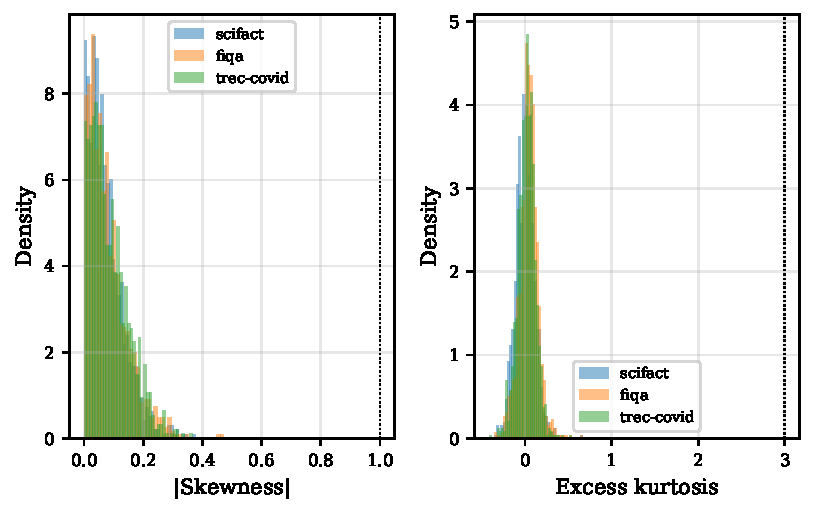
\includegraphics[width=\textwidth]{dimension_distribution.pdf}
  \caption{Verteilung der Schiefe und Kurtosis über alle 1024 Dimensionen für die drei Datensätze. Die gestrichelten Linien markieren die Schwellwerte $|\text{skew}| = 1{,}0$ und $\text{kurtosis} = 3{,}0$, ab denen Quantisierungsprobleme zu erwarten wären.}
  \label{fig:dimension_distribution}
\end{figure}
%
Die Ergebnisse sind über alle drei Datensätze bemerkenswert konsistent.
Keine einzige der 3072 untersuchten Dimensionen ($3 \times 1024$) überschreitet die Schwellwerte für problematische Schiefe oder Kurtosis.
Die maximale Schiefe liegt bei 0{,}471 (FiQA), also weniger als der Hälfte des Schwellwerts.
Die maximale Kurtosis beträgt 0{,}665 (FiQA), was einer nur leicht leptokurtischen Verteilung entspricht, die weit entfernt von problematischem Heavy-Tail-Verhalten ist.
%
\paragraph{Interpretation.}
Die nahezu symmetrischen Verteilungen um Null haben zwei konkrete Implikationen.
%
Erstens liegt der Vorzeichenschwellwert $x_i = 0$ der Binarisierung nahe am informationstheoretisch optimalen Punkt.
Bei einer symmetrischen Verteilung teilt der Schwellwert~0 die Wahrscheinlichkeitsmasse annähernd in zwei gleich große Hälften, was die Entropie des resultierenden Bits maximiert.
Die in der Methodik formulierte Erwartung, dass schiefe Dimensionen bei der Binarisierung mehr Fehler verursachen sollten, lässt sich hier nicht prüfen, da keine solchen Dimensionen existieren.
Das Fehlen schiefer Dimensionen ist jedoch selbst ein Ergebnis: Es zeigt, dass \texttt{bge-large-en-v1.5} einen für Binarisierung günstigen Raum erzeugt.
%
Zweitens bedeutet die niedrige Kurtosis, dass keine Dimension Ausreißer aufweist, die bei uniformer Quantisierung mit wenigen Stufen (etwa 4~Stufen bei 2-Bit) zu großen Fehlern führen würden.
Die uniforme Stufenverteilung von TurboQuant ist damit für diesen Raum gut geeignet.
%
Die Konsistenz über drei unterschiedliche Domänen (Naturwissenschaft, Finanz, Biomedizin) deutet darauf hin, dass diese Eigenschaften vom Modell und nicht vom Datensatz bestimmt werden.
Dies ist plausibel, da das Training über diverse Korpora hinweg eine symmetrische Nutzung des Raums erzwingt.
%
\subsection{Intrinsische Dimensionalität}
\label{sec:ergebnisse_intdim}
%
Tabelle~\ref{tab:phase1_intdim} stellt die Schätzungen der intrinsischen Dimensionalität gegenüber.
Das zugehörige PCA-Varianzspektrum und die kumulative erklärte Varianz sind in den Abbildungen~\ref{fig:pca_variance_spectrum} und~\ref{fig:pca_cumulative_variance} dargestellt.
%
\begin{table}[htbp]
  \centering
  \caption{Intrinsische Dimensionalität: TwoNN (lokale Mannigfaltigkeitsstruktur) und PCA (globale lineare Dimensionalität, 95\% erklärte Varianz). Ergänzend die kumulative Varianz bei ausgewählten Komponentenzahlen.}
  \label{tab:phase1_intdim}
  \begin{tabular}{lccccc}
    \toprule
    Datensatz & TwoNN & PCA$_{95\%}$ & $V(50)$ & $V(100)$ & $V(256)$ \\
    \midrule
    SciFact     & 13{,}2 & 390 & 50{,}0\% & 65{,}2\% & 87{,}4\% \\
    FiQA        & 22{,}1 & 395 & 52{,}7\% & 67{,}0\% & 87{,}8\% \\
    TREC-COVID  & 11{,}1 & 417 & 50{,}0\% & 63{,}8\% & 85{,}4\% \\
    \bottomrule
  \end{tabular}
\end{table}
%
\begin{figure}[htbp]
  \centering
  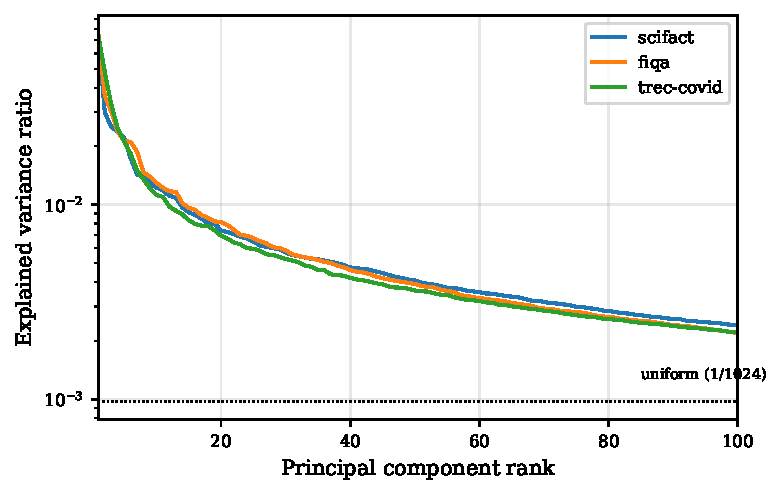
\includegraphics[width=\textwidth]{pca_variance_spectrum.pdf}
  \caption{PCA-Varianzspektrum: Erklärte Varianz pro Hauptkomponente (absteigende Reihenfolge). Der schnelle Abfall der ersten Komponenten gefolgt von einem langen, flachen Schwanz zeigt die typische Varianzkonzentration in hochdimensionalen Embedding-Räumen.}
  \label{fig:pca_variance_spectrum}
\end{figure}
%
\begin{figure}[htbp]
  \centering
  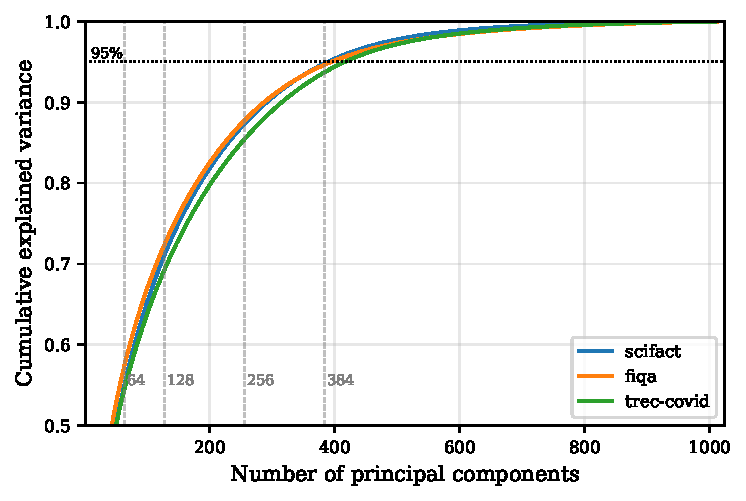
\includegraphics[width=\textwidth]{pca_cumulative_variance.pdf}
  \caption{Kumulative erklärte Varianz als Funktion der Komponentenzahl. Die horizontale Linie markiert 95\%. Die vertikalen Markierungen zeigen die evaluierten PCA-Dimensionen $d \in \{64, 128, 256, 384, 512, 768, 1024\}$.}
  \label{fig:pca_cumulative_variance}
\end{figure}
%
\paragraph{Diskrepanz zwischen lokaler und globaler Schätzung.}
Die auffälligste Beobachtung ist die starke Divergenz zwischen den beiden Schätzern.
TwoNN schätzt die lokale Mannigfaltigkeitsdimension auf 11--22, während PCA~390--417 Komponenten für 95\% Varianz benötigt.
Diese Diskrepanz beträgt mehr als eine Größenordnung und ist kein Artefakt, sondern inhaltlich interpretierbar.
%
TwoNN misst die lokale Freiheitsgrade der Datenmannigfaltigkeit: Wie viele unabhängige Richtungen existieren in der unmittelbaren Umgebung eines Punktes?
Der niedrige Wert (11--22) zeigt, dass die Dokumente lokal auf einer niedrigdimensionalen Mannigfaltigkeit liegen.
Semantisch ähnliche Dokumente unterscheiden sich nur entlang weniger Achsen.
%
PCA misst hingegen die globale lineare Dimensionalität: Wie viele orthogonale Richtungen sind nötig, um die Gesamtstreuung aller Punkte zu erfassen?
Der hohe Wert (390--417) zeigt, dass die Mannigfaltigkeit zwar lokal niedrigdimensional ist, aber global viele verschiedene Richtungen einnimmt.
Dies entspricht dem Bild einer gekrümmten Mannigfaltigkeit, die zwar lokal flach ist, aber in einen hochdimensionalen Raum eingebettet ist und dort viele verschiedene Orientierungen annimmt.
%
\paragraph{Implikationen für die Dimensionsreduktion.}
Aus den PCA-Ergebnissen lassen sich quantitative Vorhersagen für die nachfolgenden Phasen ableiten:
\begin{itemize}
  \item \textbf{$d = 384$:} Mit 384 Komponenten werden je nach Datensatz 93--94\% der Varianz erhalten (interpoliert aus den Werten für $V(256)$ und $V(\text{PCA}_{95\%})$).
Eine moderate Qualitätsreduktion ist zu erwarten, aber keine katastrophale.
  \item \textbf{$d = 256$:} Bei 256 Komponenten verbleiben 85--88\% der Varianz.
Hier beginnt der Bereich, in dem substantielle Information verloren geht.
  \item \textbf{$d = 64$:} Bei 64 Komponenten verbleiben nur ca. 40\% der Varianz.
Ein massiver Qualitätsverlust ist zu erwarten.
\end{itemize}
%
\paragraph{Implikationen für die Quantisierung.}
Die niedrige lokale Dimensionalität (TwoNN $\approx$ 11--22) hat eine weitere Konsequenz.
Sie bedeutet, dass die lokale Nachbarschaftsstruktur, die für Retrieval entscheidend ist, durch relativ wenige effektive Dimensionen bestimmt wird.
Quantisierung, die jede Dimension unabhängig behandelt, kann daher einen substantiellen Teil der Bitbreite auf redundante Dimensionen verwenden, ohne die relevante lokale Struktur zu beschädigen.
Dies legt nahe, dass selbst aggressive Quantisierung (2-Bit, 1-Bit) die \emph{lokale} Nachbarschaftsstruktur besser erhalten könnte als die \emph{globale} Distanzstruktur, da erstere von weniger effektiven Dimensionen abhängt.
Diese Hypothese wird in Phase~3 empirisch geprüft.
%
\subsection{Zusammenfassung und Vorhersagen}
\label{sec:ergebnisse_phase1_vorhersagen}
%
Die Charakterisierung ergibt ein konsistentes Bild: Der Embedding-Raum von \texttt{bge-large-en-v1.5} besitzt drei Eigenschaften, die Quantisierung systematisch begünstigen:
\begin{enumerate}
  \item \textbf{Perfekte Normierung} -- die Binarisierung verliert keine Norminformation.
  \item \textbf{Symmetrische, leicht-schwänzige Dimensionen} -- der Vorzeichenschwellwert liegt optimal, und uniforme Quantisierung verursacht keine Ausreißer-induzierten Fehler.
  \item \textbf{Hohe Redundanz} -- die intrinsische Dimensionalität liegt weit unter der nominalen, sodass Kompression über beide Achsen (Bittiefe und Dimensionszahl) möglich ist.
\end{enumerate}
%
Daraus ergeben sich spezifische, testbare Vorhersagen für die nachfolgenden Phasen:
\begin{itemize}
  \item Selbst die naive Binarisierung sollte aufgrund der günstigen Raumeigenschaften eine nicht-triviale Distanz- und Nachbarschaftserhaltung zeigen.
  \item Der Vorteil von TurboQuant gegenüber naiver Quantisierung sollte moderat ausfallen, da die Varianzumverteilung durch Rotation in einem bereits gleichmäßig genutzten Raum weniger Verbesserungspotenzial hat.
  \item PCA-Reduktion auf $d \geq 384$ sollte bei allen Quantisierungsstufen nur marginale Qualitätsverluste verursachen.
  \item Die stärksten Qualitätseinbrüche werden bei $d \leq 128$ erwartet, wo mehr als 30\% der Varianz verloren gehen.
\end{itemize}
%
Ob diese Vorhersagen zutreffen, wird in den Phasen~2 bis~4 empirisch überprüft.
%
\printbibliography
%
\appendix
\addchap{Anhang}
\KOMAoptions{open=any}
%
\chapter*{Eigenständigkeitserklärung}
%
Wir versichern, die von uns vorgelegte Arbeit selbstständig verfasst zu haben.
Alle Stellen, die wörtlich oder sinngemäß aus veröffentlichten oder nicht veröffentlichten Arbeiten anderer entnommen sind, haben wir als entnommen kenntlich gemacht.
Sämtliche Quellen und Hilfsmittel, die wir für die Arbeit benutzt haben, sind angegeben.
Die Arbeit hat mit gleichem Inhalt bzw.\ in wesentlichen Teilen noch keiner anderen Prüfungsbehörde vorgelegen.
%
\section*{Verwendete Hilfsmittel}
%
Bei der Erstellung dieser Arbeit wurden die folgenden KI-gestützten Werkzeuge als technische Hilfsmittel eingesetzt:
%
\begin{itemize}
  \item \textbf{Google Gemini} (Google DeepMind, 2026)
  \item \textbf{Kiro CLI} (Amazon, 2026)
  \item \textbf{OpenAI Codex / ChatGPT} (OpenAI, 2026)
\end{itemize}
%
Die genannten Werkzeuge wurden gleichermaßen für Recherche, Formulierung und Strukturierung der Projektarbeit, für die Codeentwicklung sowie für die Literaturrecherche eingesetzt.
Die inhaltliche Verantwortung, die wissenschaftliche Argumentation, die Konzeption des Experiments sowie die Interpretation der Ergebnisse liegen vollständig bei den Verfassern.
Alle von KI-Werkzeugen generierten Inhalte wurden kritisch geprüft, überarbeitet und in eigener Verantwortung in die Arbeit integriert.
%
\par\vspace{\fill}
%
\noindent\begin{minipage}{\textwidth}
\vspace{1.5cm}
\noindent\rule{5cm}{0.4pt}\hfill\rule{7cm}{0.4pt}\\[2pt]
\noindent\makebox[5cm][c]{Ort, Datum}\hfill\makebox[7cm][c]{Unterschrift}

\vspace{1cm}

\noindent\rule{5cm}{0.4pt}\hfill\rule{7cm}{0.4pt}\\[2pt]
\noindent\makebox[5cm][c]{Ort, Datum}\hfill\makebox[7cm][c]{Unterschrift}

\vspace{1cm}

\noindent\rule{5cm}{0.4pt}\hfill\rule{7cm}{0.4pt}\\[2pt]
\noindent\makebox[5cm][c]{Ort, Datum}\hfill\makebox[7cm][c]{Unterschrift}
\end{minipage}

%
%
\end{document}
